% %*----------- SLIDE -------------------------------------------------------------
% \begin{frame}[t]{Accuracy results } %pensar no que colocar
%         \begin{table}[]
%                 \scalefont{0.55}
%                 \begin{tabular}{|c|c|c|c|c|c|c|c|c|c|}
%                 \hline
%                 \multicolumn{10}{|c|}{\textbf{ACCURACY RESULTS (METHODS AND DATASETS) (\%)}}     \\ \hline
%                 \textbf{Method / Dataset} &
%                   \textbf{\begin{tabular}[c]{@{}c@{}}PASCAL \\ VOC-2012\end{tabular}} &
%                   \textbf{\begin{tabular}[c]{@{}c@{}}Pascal- Person- \\ Part\end{tabular}} &
%                   \textbf{CamVid} &
%                   \textbf{CityScapes} &
%                   \textbf{\begin{tabular}[c]{@{}c@{}}Stanford \\ Background\end{tabular}} &
%                   \textbf{SiftFlow} &
%                   \textbf{SUN3D} &
%                   \textbf{\begin{tabular}[c]{@{}c@{}}ShapeNet \\ Part\end{tabular}} &
%                   \textbf{\begin{tabular}[c]{@{}c@{}}Youtube- \\ Objects\end{tabular}} \\ \hline
%                 \textbf{PSPNet}            & 85,4 &       &       &       &       &  &       &       &       \\ \hline
%                 \textbf{DeepLab}           &      & 64,94 &       &       &       &  &       &       &       \\ \hline
%                 \textbf{DAG-RNN}           &      &       & 91,60 &       &       &  &       &       &       \\ \hline
%                 \textbf{rCNN}              &      &       &       &       & 80,20 &  &       &       &       \\ \hline
%                 \textbf{LSTM-CF}           &      &       &       &       &       &  & 58,50 &       &       \\ \hline
%                 \textbf{PointNet}          &      &       &       &       &       &  &       & 83,70 &       \\ \hline
%                 \textbf{PointNet++}        &      &       &       &       &       &  &       & 85,10 &       \\ \hline
%                 \textbf{DGCNN}             &      &       &       &       &       &  &       & 85,10 &       \\ \hline
%                 \textbf{Clockwork Convent} &      &       &       &       &       &  &       &       & 68,50 \\ \hline
%                 \textbf{SegmPred}          &      &       &       & 59,40 &       &  &       &       &       \\ \hline
%                 \end{tabular}
%                 \caption{Accuracy results for the most relevant methods and dataset. \cite{garcia2018survey}}
%                 \label{tab:accuracy_results}
%                 \end{table}
% \end{frame}

%*----------- SLIDE -------------------------------------------------------------
\begin{frame}[t]{Wich cases doesn't apply deep learning?} %usar limitations?
        \begin{columns}[c]
                \column{.05\textwidth}
                \column{.6\textwidth}
                        For \textbf{high perfomance}, deep networks require \textbf{extremely large} datasets.  
                        \newline
                        \newline
                        It's \textbf{expensive} to get data, computer power and hiring researchers.
                        \newline
                        \newline
                        Deep networks \textbf{aren't easily interpreted} as classical Machine Learning algorithms.
                \column{.35\textwidth}
                    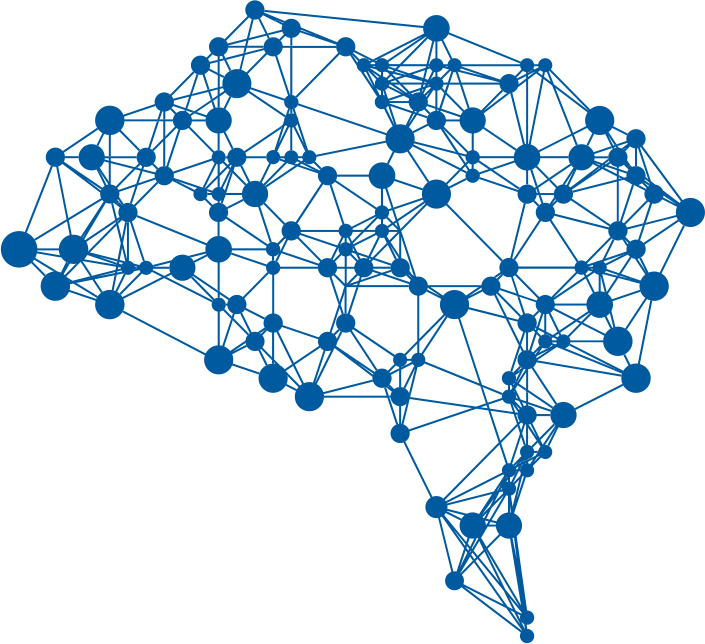
\includegraphics[width=0.9\textwidth]{dnn}
            \end{columns}
        
    
\end{frame}
%-

%*----------- SLIDE -------------------------------------------------------------
\begin{frame}[t]{Advantages to use Deep learning against to Classical methods} 
        \begin{columns}[c]
                \column{.05\textwidth}
                \column{.6\textwidth}
                \newline
                \newline
                \textbf{Better} performance (accuracy results)
                \newline
                \newline
                More data works to DP \textbf{but not} with CML
                \newline
                \newline
                DP \textbf{no need} for feature engineering
                \newline
                \newline
                It's \textbf{adaptable} to differents domains and applications
                \newline
                \newline
                \column{.35\textwidth}
                        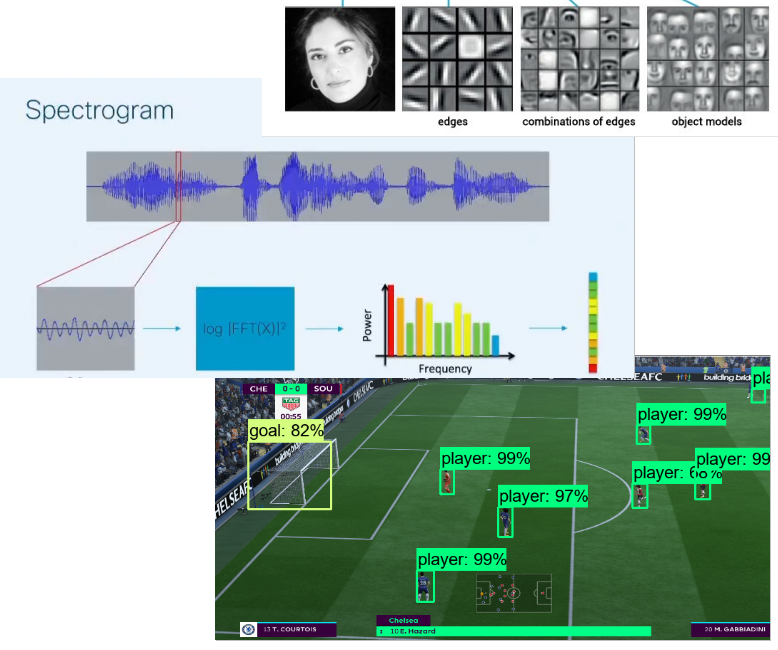
\includegraphics[width=0.9\textwidth]{example}
        \end{columns}
       
\end{frame}
%-


%*----------- SLIDE -------------------------------------------------------------
\begin{frame}[t]{Advantages to use Classical methods against to  Deep learning} 
        \begin{columns}[c]
                \column{.05\textwidth}
                \column{.6\textwidth}
                \newline
                \newline
                Works better with \textbf{small dataset}
                \newline
                \newline
                \textbf{Low} computional and financial cost
                \newline
                \newline
                The algorithms it's \textbf{easier} to understand and interpret
                \newline
                \newline
                \column{.35\textwidth}
        \end{columns}
       
\end{frame}